\documentclass[11pt]{beamer}
\usepackage{helvet} %font
\beamertemplatenavigationsymbolsempty
\usetheme{JuanLesPins}
\usefonttheme{structurebold}

\usepackage[french]{babel}
\usepackage[utf8]{inputenc}
\usepackage[T1]{fontenc}
\usepackage{amssymb,amsmath}
\usepackage{tikz}
\usepackage{geometry}
\usepackage{xcolor,colortbl}
\usetikzlibrary{arrows,positioning}
\usepackage{listings}

\AtBeginSubsection[]
{
   \begin{frame}
	\small \tableofcontents[currentsection]
   \end{frame}
}

\newenvironment{slide}[1]{%
\begin{frame}[environment=slide]
\frametitle{#1}
}{%
\end{frame}
}
\setbeamercolor{structure}{fg=red}
\setbeamercolor{frametitle}{bg=black,fg=white}
\definecolor{gris}{gray}{0.6}
\definecolor{grisclair}{gray}{0.9}

\newtheorem{exercice}{Exercice}

\title{Machine Learning - Introduction}
\author{Nicolas Bourgeois}
\date{}

\newcommand{\Python}[1]{
	{\small	\lstinputlisting[language=Python]{./#1.py}}
}
\newenvironment{pyenvsmall}
	{ \ttfamily \tiny }
	{\par  }

\newcommand{\Pythonsmall}[1]{
	{\scriptsize \lstinputlisting[language=Python]{./#1.py}}
}
\newcommand{\elimine}[1]{{\textcolor{lightgray}{#1}}}


\begin{document}

\begin{frame}
\maketitle
\end{frame}

\begin{frame}
\small
\tableofcontents
\end{frame}

\section{Motivation}

\subsection{Exemples}

\begin{slide}{}

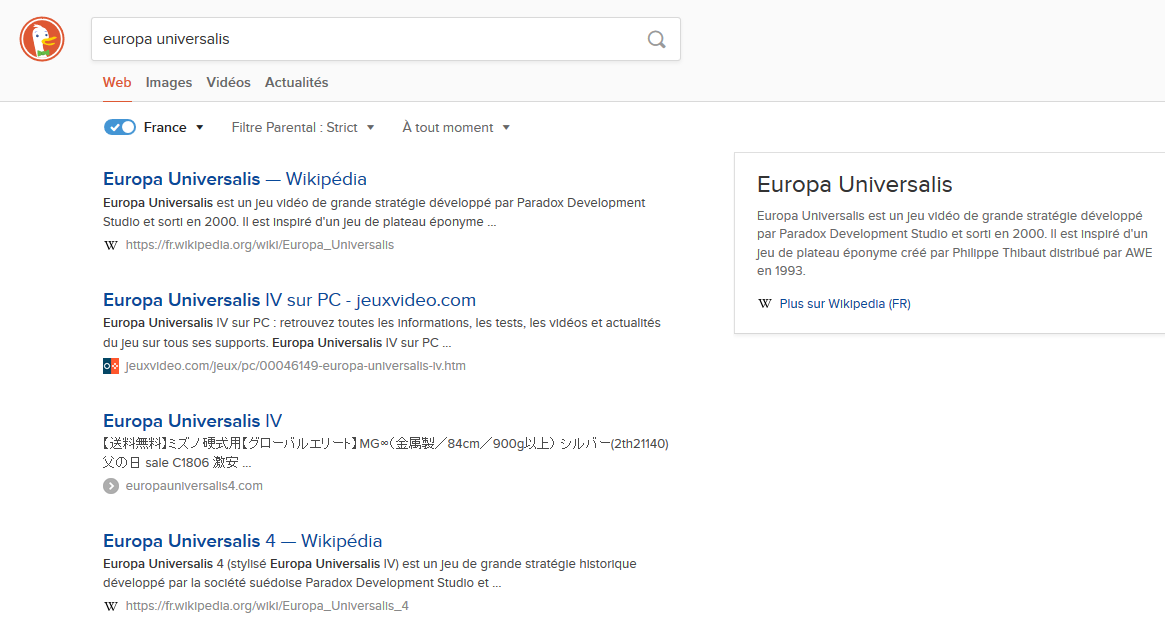
\includegraphics[scale=0.25]{A1ranking}

\end{slide}

\begin{slide}{}

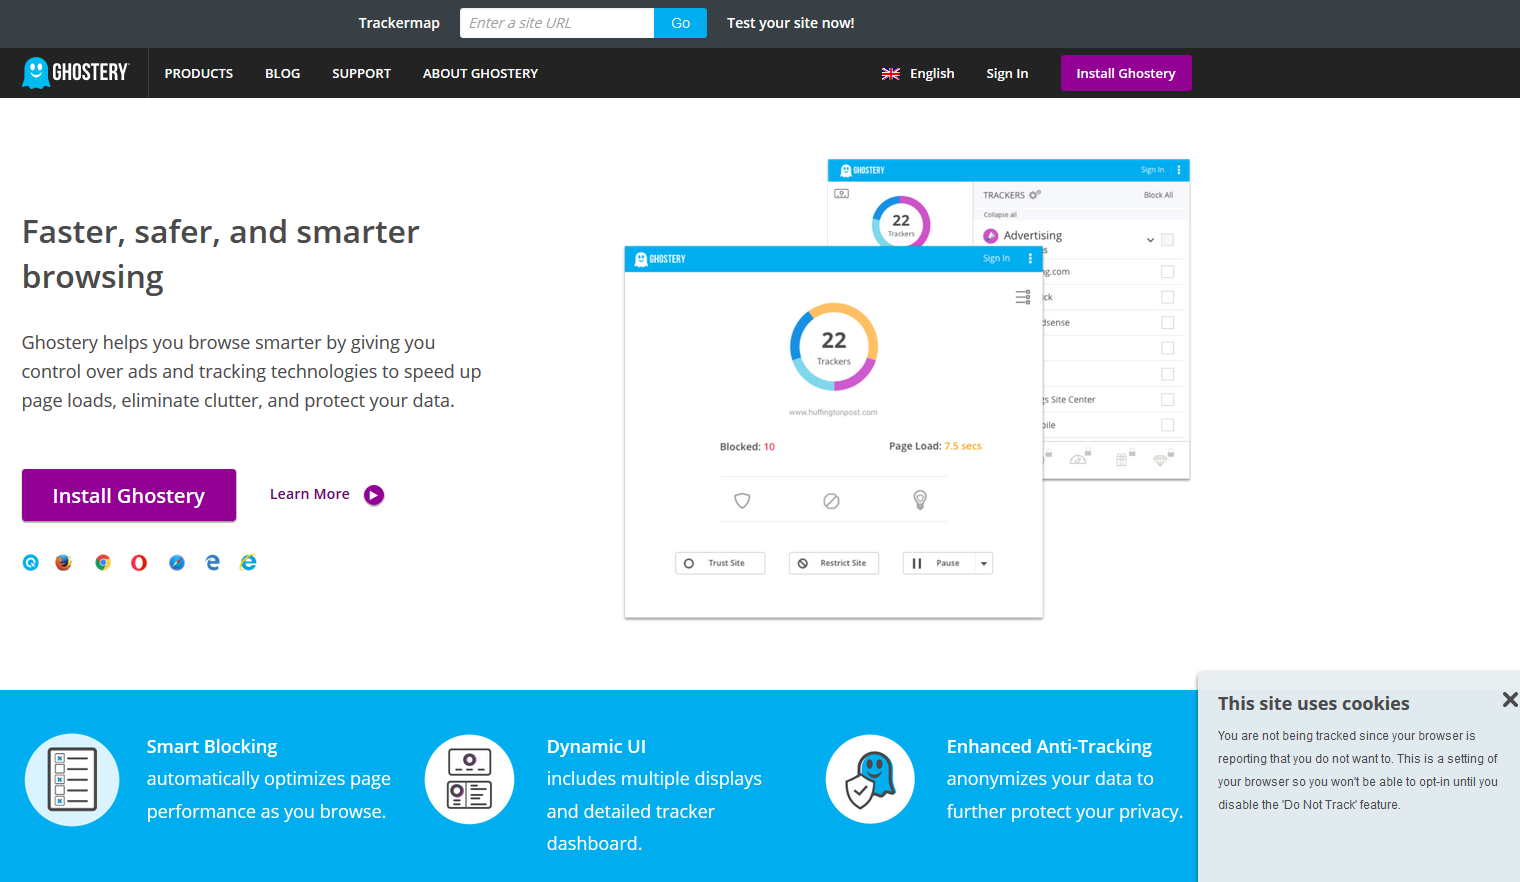
\includegraphics[scale=0.2]{A2targeting}

\end{slide}

\begin{slide}{}

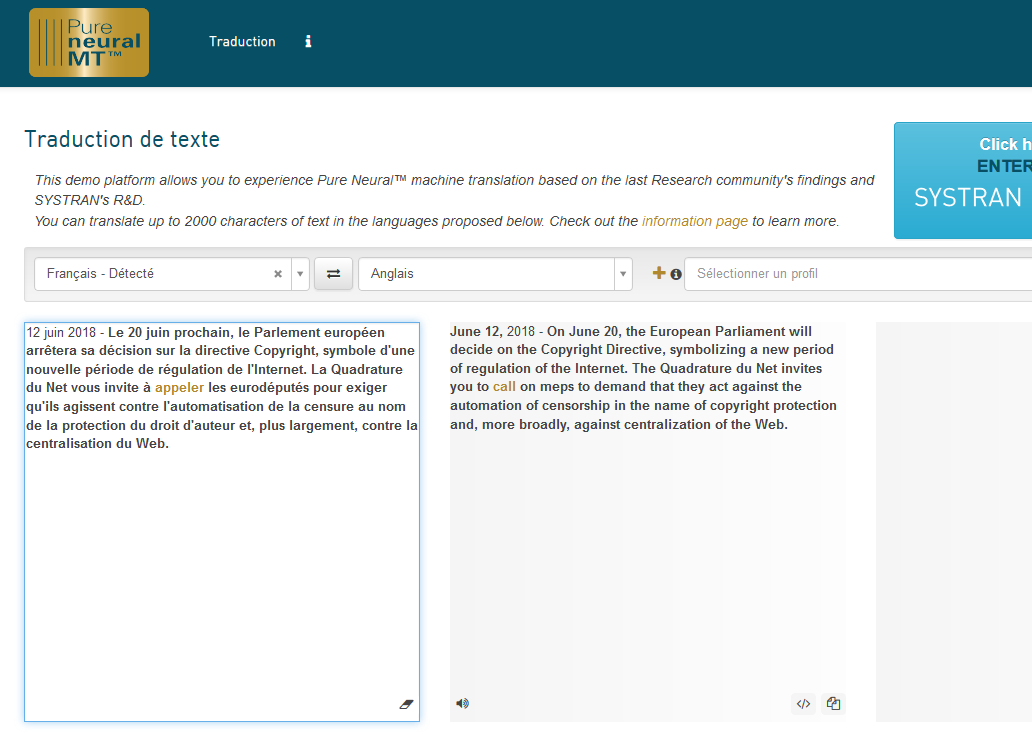
\includegraphics[scale=0.3]{A3tnl}

\end{slide}

\begin{slide}{}

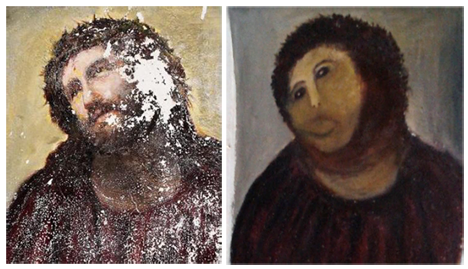
\includegraphics[scale=0.5]{A4facerecognition}

\end{slide}

\begin{slide}{}


\includegraphics[scale=0.75]{A5imagerecognition}

\end{slide}

\begin{slide}{}

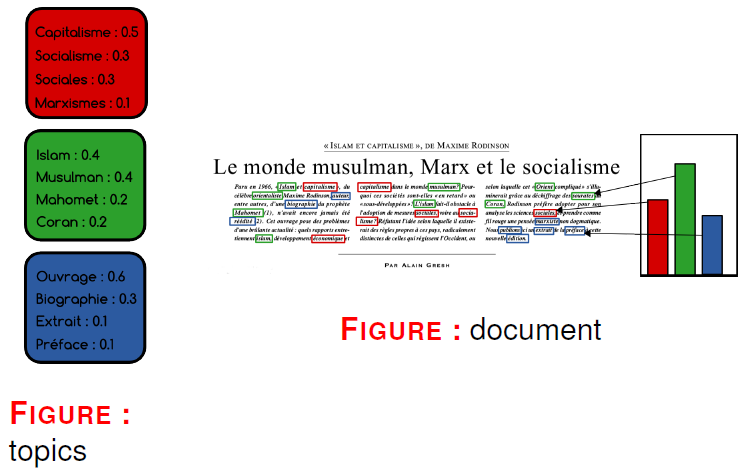
\includegraphics[scale=0.35]{A6topicrecognition}

\end{slide}

\begin{slide}{}

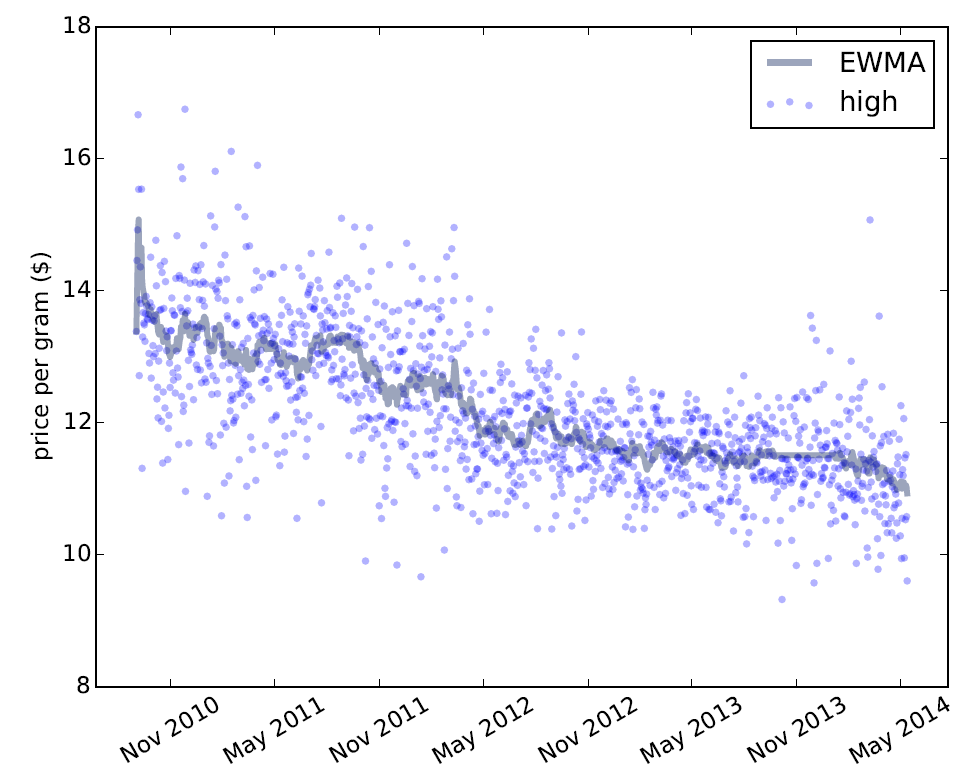
\includegraphics[scale=0.25]{A7regression}

\end{slide}

\begin{slide}{}

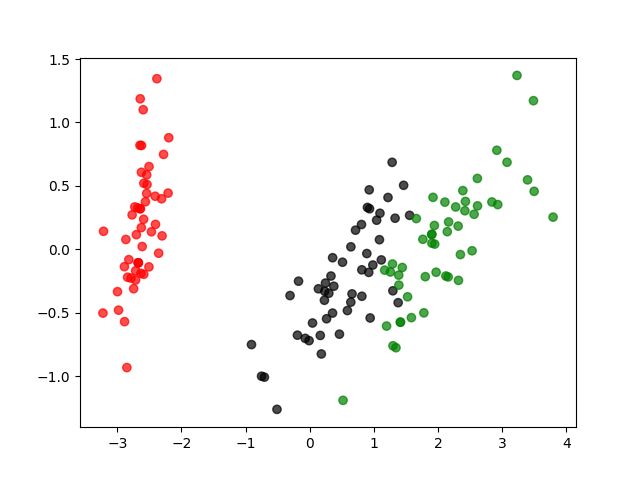
\includegraphics[scale=0.5]{A8classif}

\end{slide}

\begin{slide}{}


\includegraphics[scale=0.25]{A9videogames}

\end{slide}

\subsection{L'apprentissage : idée générale}

\begin{slide}{Environnement}
Python 3, avec les librairies suivantes :\\

\begin{itemize}
	\item numpy, scipy
	\item pandas
	\item matplotlib, seaborn, pygraphviz
	\item scikit-learn, tensorflow
\end{itemize}	
	
\end{slide}

\begin{slide}{Install Party Now}

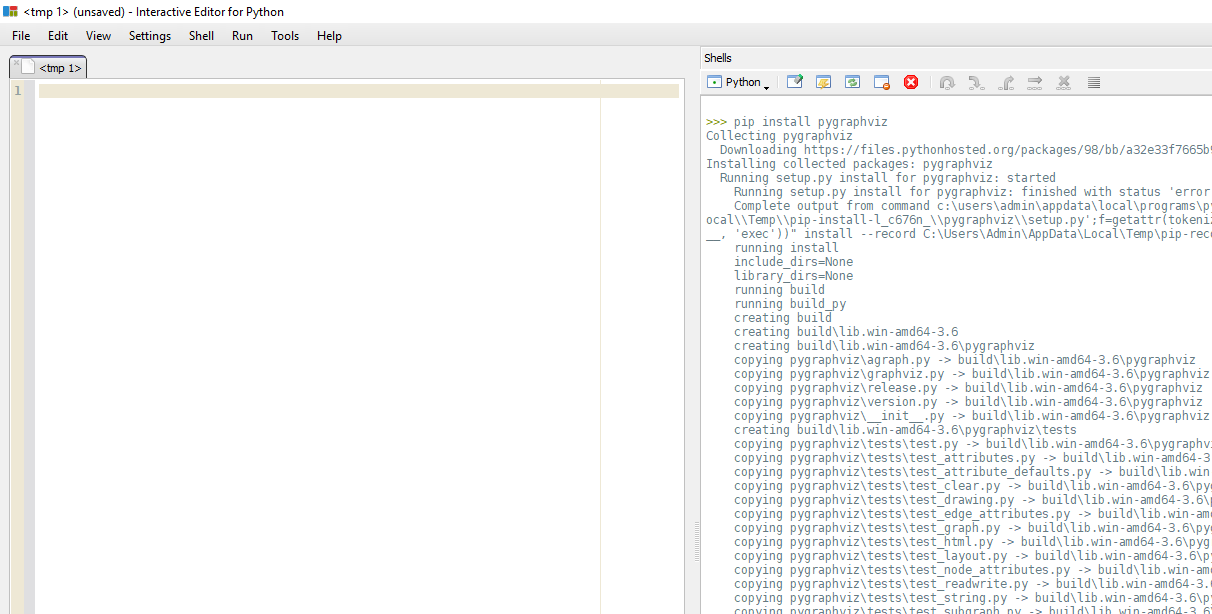
\includegraphics[scale=0.25]{pyzo}

\end{slide}

\begin{slide}{Méthode Générale (I)}

\begin{enumerate}

\item Définir (acquérir) un jeu de données
\pause
\item Préciser un objectif
\pause
\item Choisir un modèle
\pause
\item Identifier des algorithmes
\pause
\item Evaluer la performance (fiabilité)

\end{enumerate}

\end{slide}

\begin{slide}{Apprentissage Supervisé}

Observations :\\

\begin{itemize}

\item Variable empirique cible $\tilde{Y}$ (gain d'un match)
\item Variables empiriques explicatives $\tilde{X}$ (joueurs, terrain)

\end{itemize}

\pause

Hypothèses :\\

\begin{itemize}

\item $\tilde{X}$ est un ensemble d'observations lié à un processus aléatoire $X$
\item $\tilde{Y}$ est un ensemble d'observations lié à un processus aléatoire $Y$
\item il existe une relation $Y = f(X)$

\end{itemize}

\pause

Objectifs :\\

\begin{itemize}
\item Produire une fonction $\tilde{f}$ à partir de $\tilde{X}$ et $\tilde{Y}$
\item Telle que $\tilde{f}$ soit une approximation fiable de $f$
\item On pourra ainsi prédire $\tilde{Y}' = \tilde{f}(\tilde{X}')$ sur un nouvel échantillon 
\end{itemize}

\end{slide}

\begin{slide}{Apprentissage non Supervisé}

Observations :\\

\begin{itemize}

\item Variable empirique $\tilde{X}$ (caractéristiques économiques)

\end{itemize}

\pause

Hypothèses :\\

\begin{itemize}

\item $\tilde{X}$ est un ensemble d'observations lié à un processus aléatoire $X$

\end{itemize}

\pause

Objectifs :\\

\begin{itemize}
\item Caractériser autant que possible le processus $X$
\item Par exemple pour classer l'information $\tilde{X}$
\item Ou pour la visualiser
\item D'une façon qui reste fiable sur d'autres observations $\tilde{X}'$
\end{itemize}

\end{slide}

\begin{slide}{Exercice}
\begin{exercice}
Dans les exemples précédents, identifier le caractère supervisé ou non du problème et les variables en jeu.
\end{exercice}
\end{slide}


\begin{slide}{}

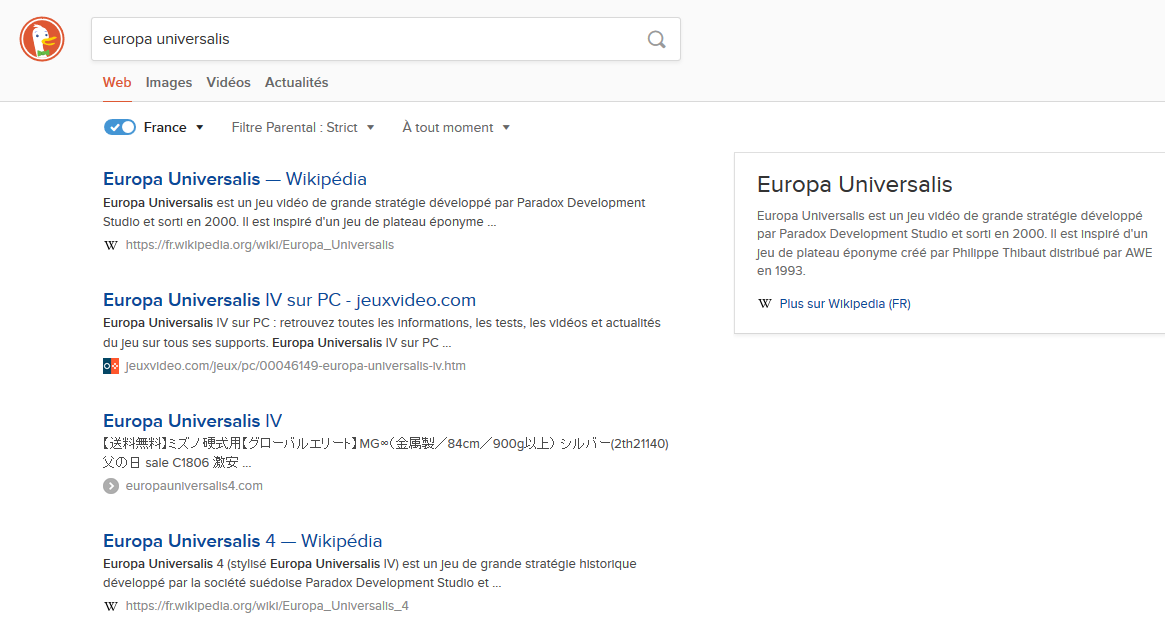
\includegraphics[scale=0.25]{A1ranking}

\end{slide}

\begin{slide}{}

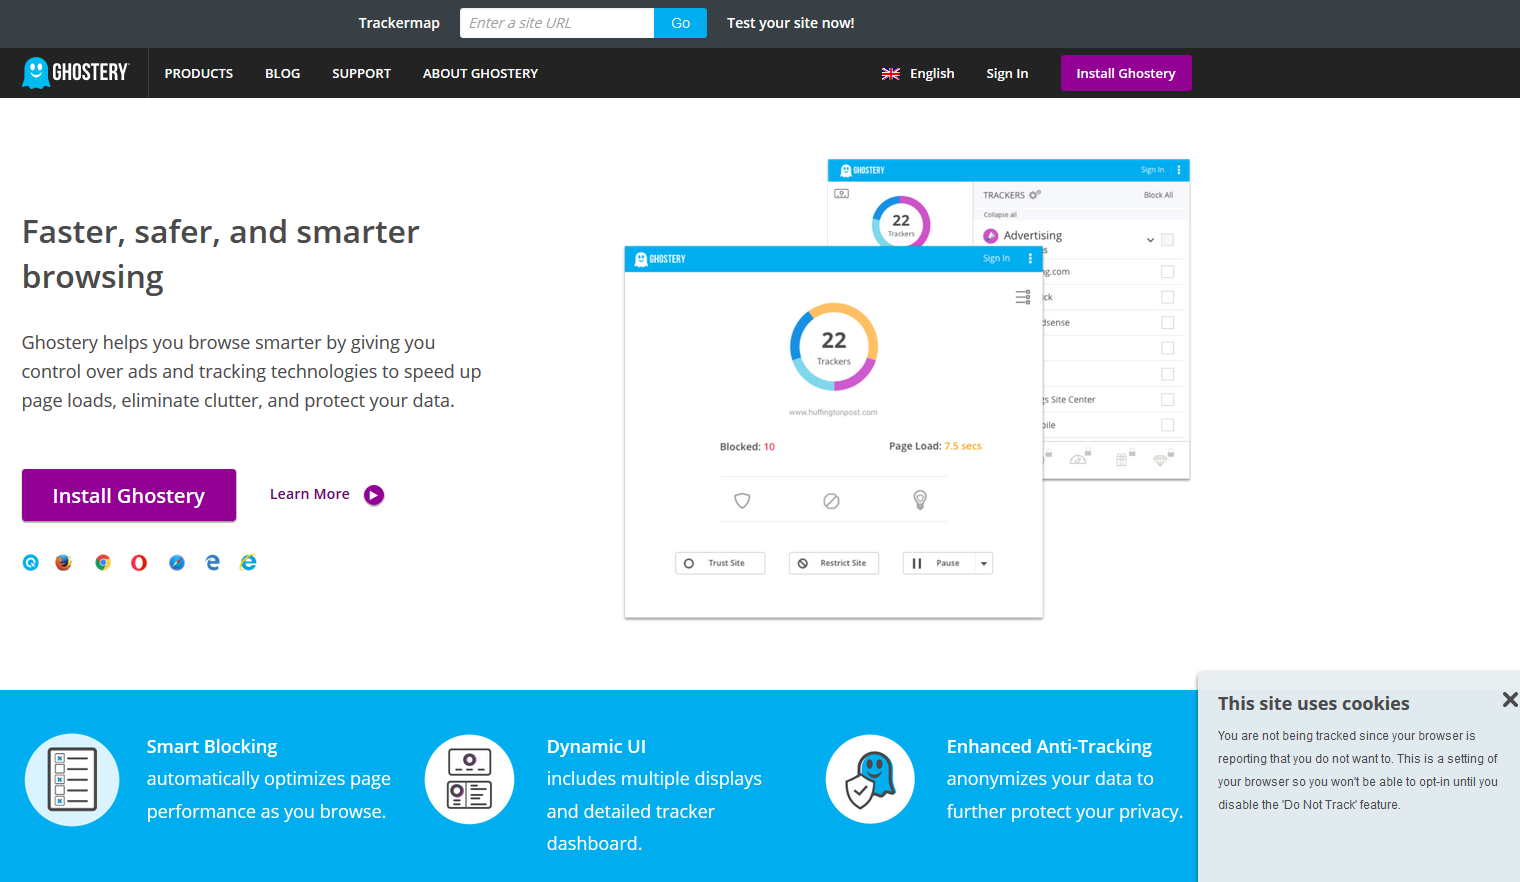
\includegraphics[scale=0.2]{A2targeting}

\end{slide}

\begin{slide}{}

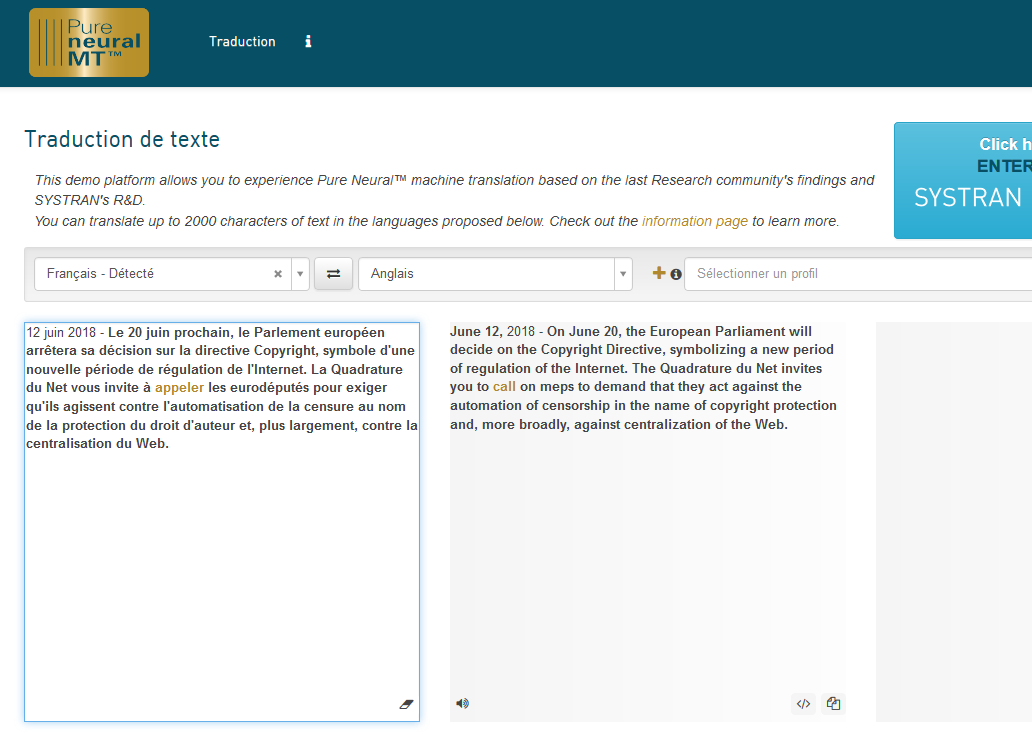
\includegraphics[scale=0.3]{A3tnl}

\end{slide}

\begin{slide}{}

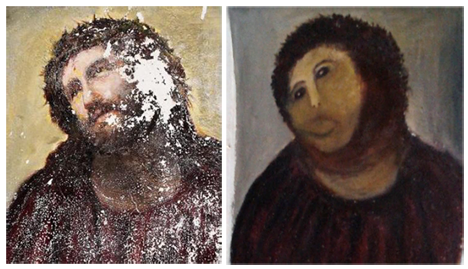
\includegraphics[scale=0.5]{A4facerecognition}

\end{slide}

\begin{slide}{}


\includegraphics[scale=0.75]{A5imagerecognition}

\end{slide}

\begin{slide}{}

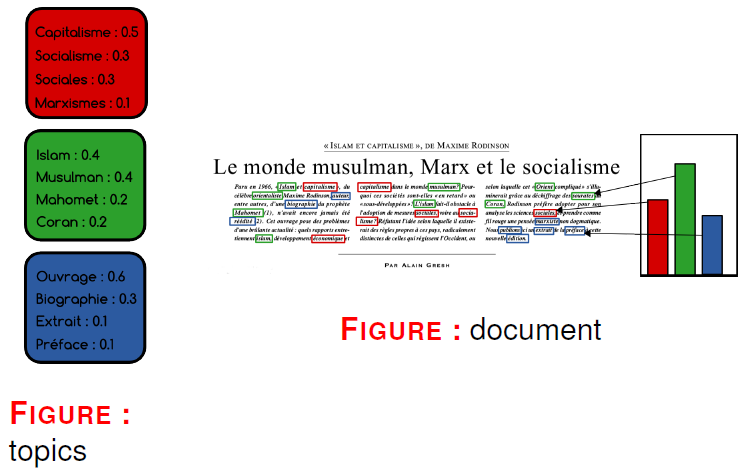
\includegraphics[scale=0.35]{A6topicrecognition}

\end{slide}

\begin{slide}{}

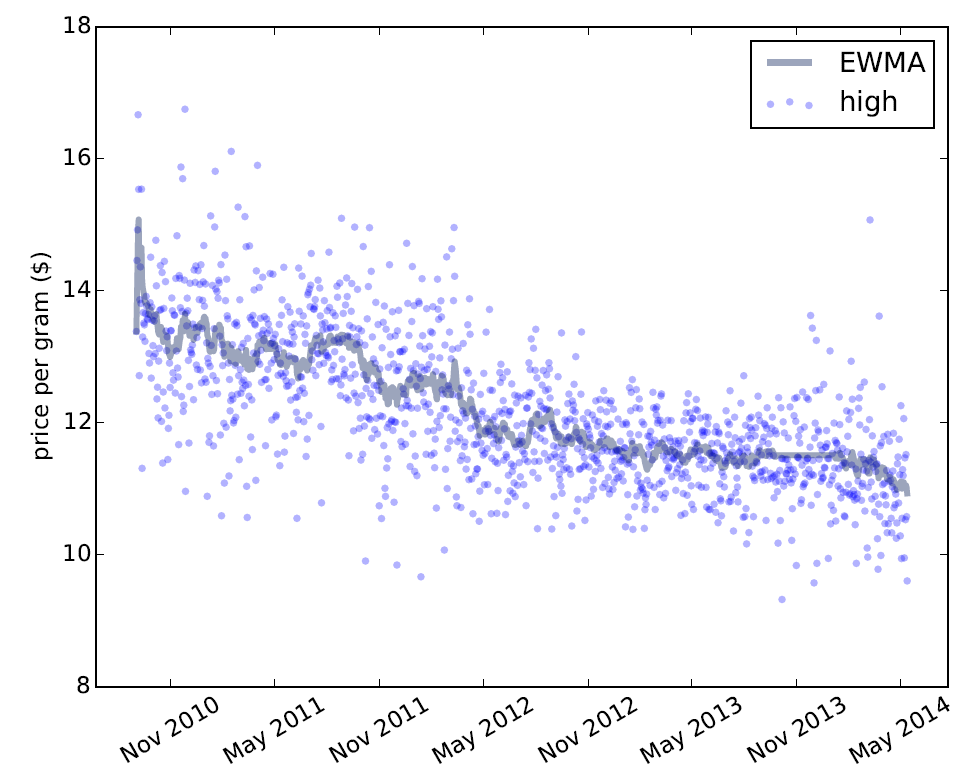
\includegraphics[scale=0.25]{A7regression}

\end{slide}

\begin{slide}{}

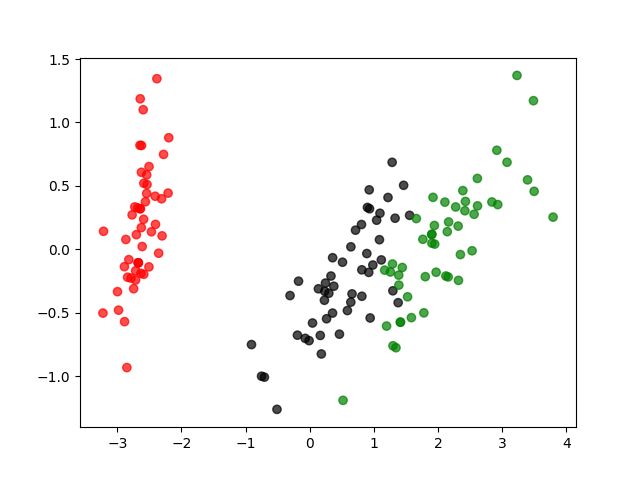
\includegraphics[scale=0.5]{A8classif}

\end{slide}

\begin{slide}{}


\includegraphics[scale=0.25]{A9videogames}

\end{slide}

\subsection{Valeur d'un résultat}

\begin{slide}{Qualité}

\begin{itemize}
	\item Adéquation de la prédiction : marge d'erreur, risque d'erreur
	\item S'évalue sur un échantillon de test différent de l'échantillon d'apprentissage
	\item Temps de calcul, vitesse de convergence
\end{itemize}

\end{slide}

\begin{slide}{Surapprentissage}

\begin{exercice}
Montrez qu'il est toujours possible de trouver un modèle parfaitement fiable sur l'échantillon d'apprentissage.
\end{exercice}

\pause

\begin{exercice}
Montrez que ce modèle peut être en fait très mauvais sur un échantillon de test.
\end{exercice}

\end{slide}

\begin{slide}{}

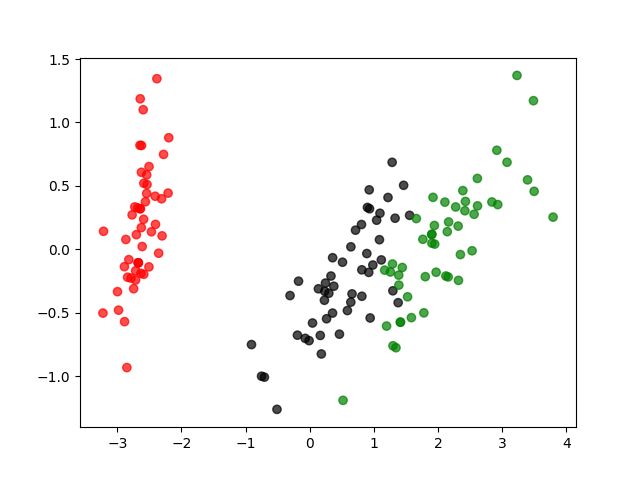
\includegraphics[scale=0.5]{A8classif}

\end{slide}


\begin{slide}{}

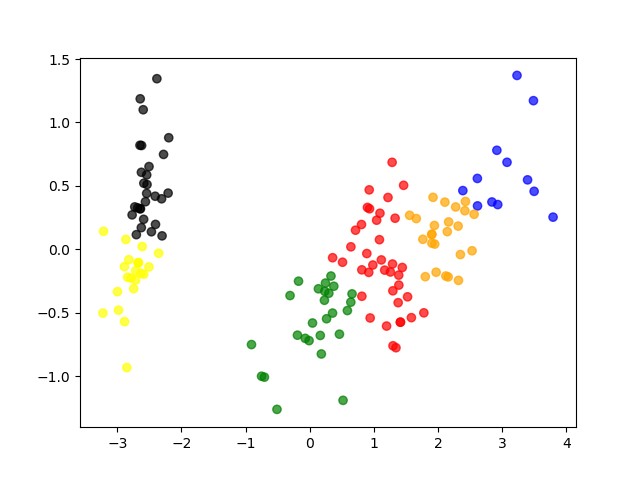
\includegraphics[scale=0.5]{iris_surapprentissage}

\end{slide}

\begin{slide}{}

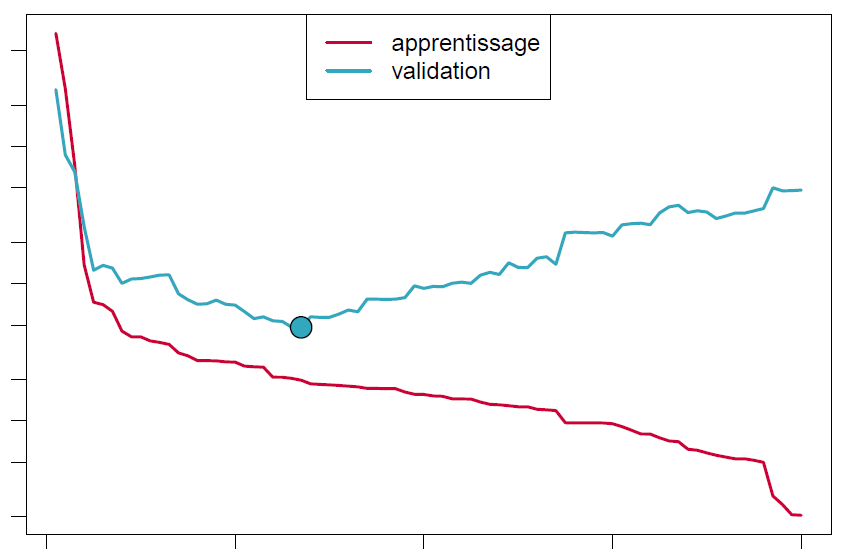
\includegraphics[scale=0.3]{testvalidation}

\end{slide}

\begin{slide}{Warnings}

\begin{exercice}
Essayez d'identifier un maximum de sources d'échec dans un processus d'apprentissage.
\end{exercice}

Solutions dans la partie 4\ldots

\end{slide}

\section{Visualisation}

\subsection{Aux origines du problème}

\begin{slide}{Des représentations naturelles ?}

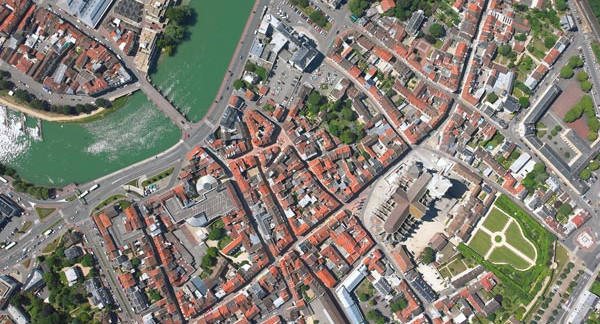
\includegraphics[scale=0.5]{meaux}


\end{slide}

\begin{slide}{Des représentations naturelles ?}
\begin{center}

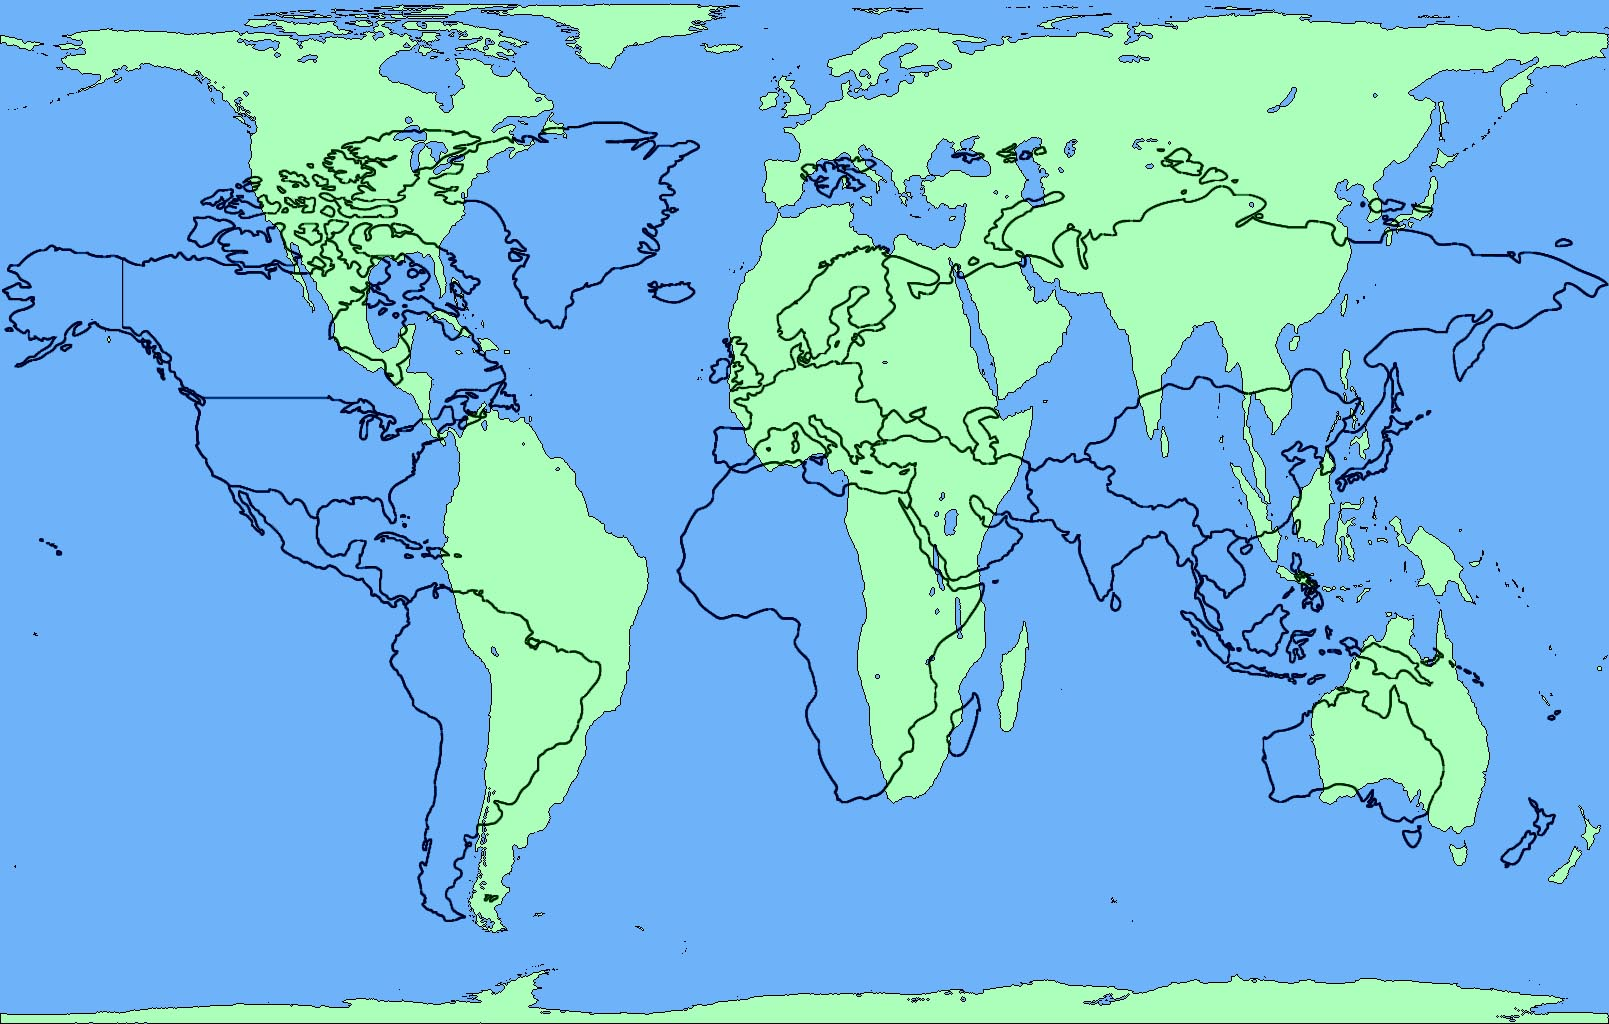
\includegraphics[scale=0.15]{projections}

\end{center}
\end{slide}

\begin{slide}{Des représentations naturelles ?}

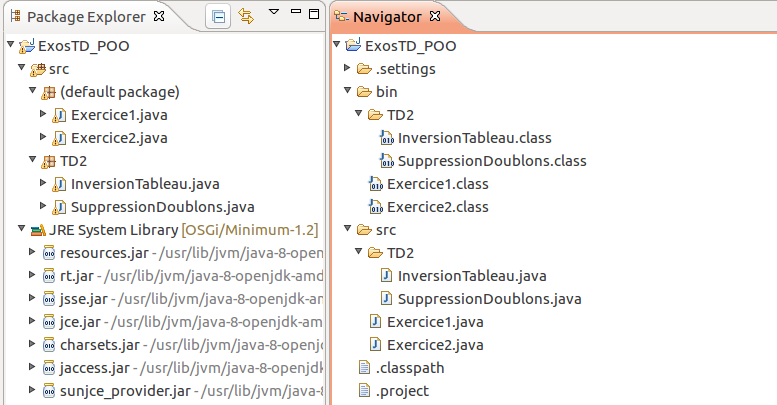
\includegraphics[scale=0.35]{files}

\end{slide}

\begin{slide}{Des représentations naturelles ?}

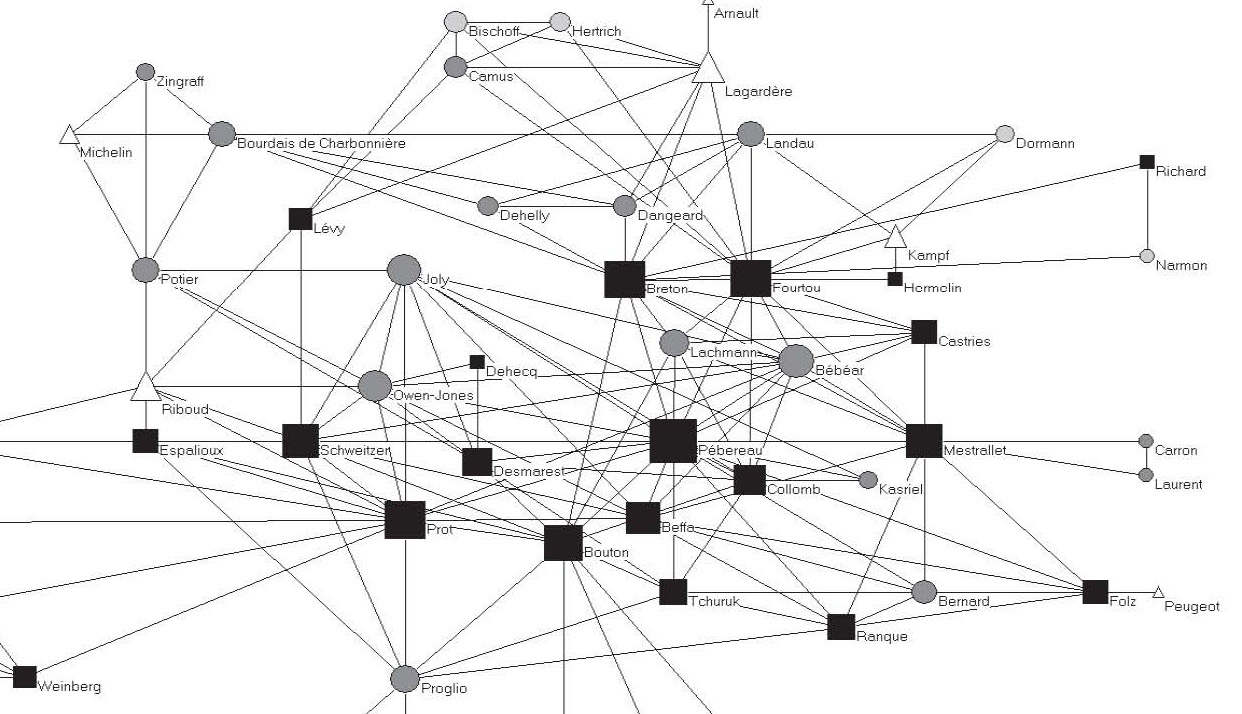
\includegraphics[scale=0.6]{dudouet}

\end{slide}

\begin{slide}{Problème: multidimensionnalité}

\begin{center}

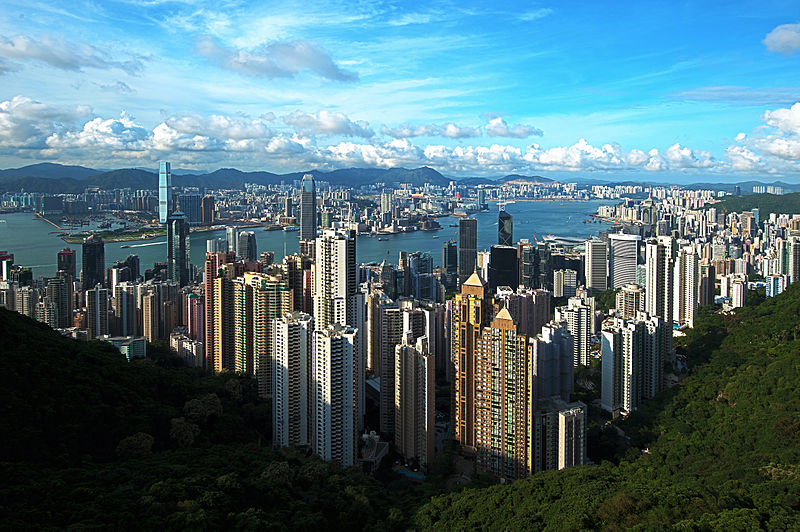
\includegraphics[scale=0.95]{hongkong}

\end{center}
\end{slide}

\begin{slide}{Problème: multidimensionnalité}

\begin{center}

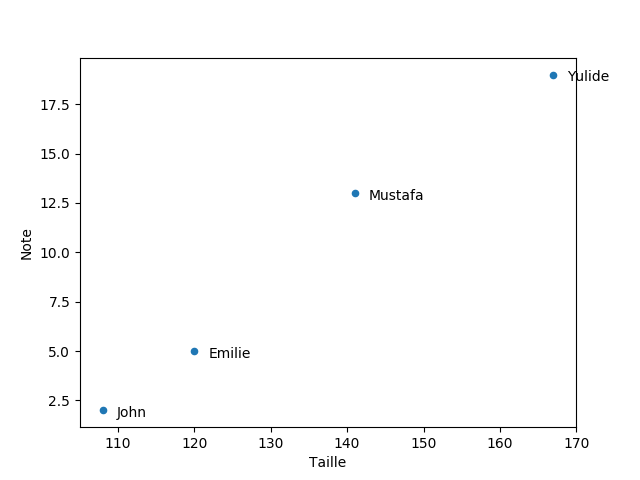
\includegraphics[scale=0.4]{plot1}

\end{center}
\end{slide}

\begin{slide}{Problème: multidimensionnalité}
\begin{center}
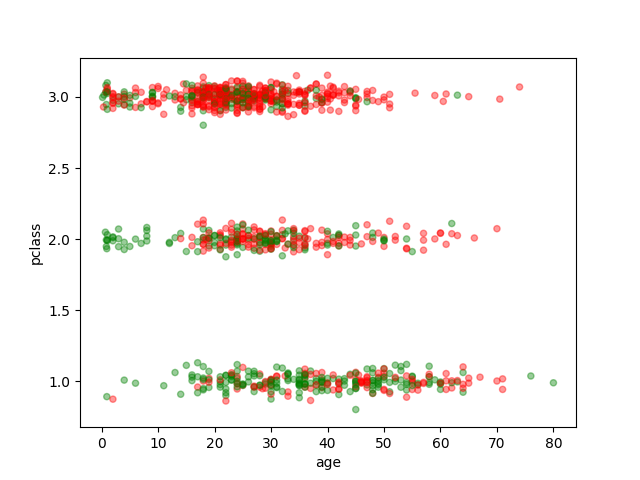
\includegraphics[scale=0.4]{titanic_plot}
\end{center}
\end{slide}

\begin{slide}{Problème: multidimensionnalité}
\begin{center}
{\tiny \input{data3.txt}}
\end{center}
\end{slide}

\begin{slide}{Problème: multidimensionnalité}
\begin{center}

\includegraphics[scale=.75]{optdigits-7}
\end{center}
\end{slide}

\subsection{Réduction dimensionnelle}

\begin{slide}{Scatter Matrix}
\begin{center}
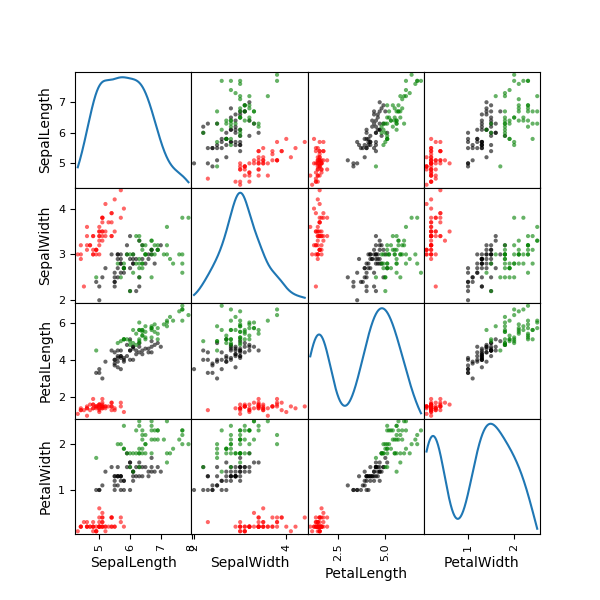
\includegraphics[scale=0.4]{iris_matrix}
\end{center}
\end{slide}

\begin{slide}{Scatter Matrix}
\begin{center}
\Python{scatter_matrix}
\end{center}
\end{slide}

\begin{slide}{Scatter Matrix}
\begin{center}
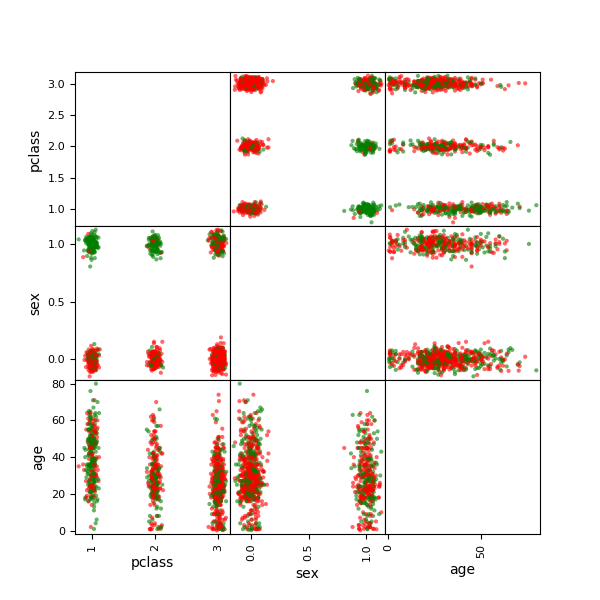
\includegraphics[scale=0.4]{titanic_matrix}
\end{center}
\end{slide}

\begin{slide}{ACP}
\begin{center}
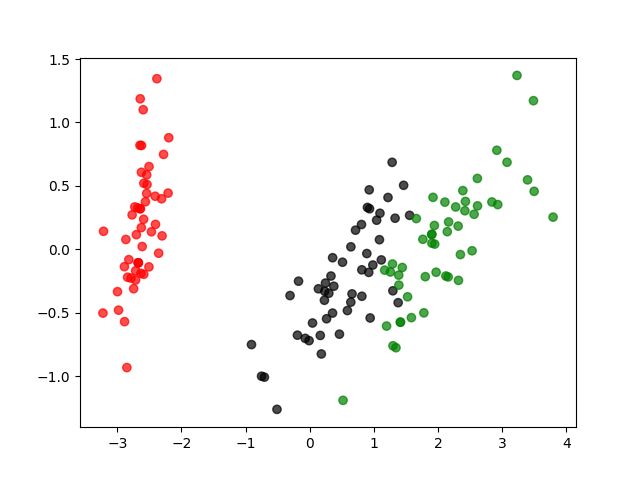
\includegraphics[scale=0.4]{iris_acp}
\end{center}
\end{slide}

\begin{slide}{ACP}
\begin{center}
\Python{acp}
\end{center}
\end{slide}

\begin{slide}{ACP}
\begin{center}
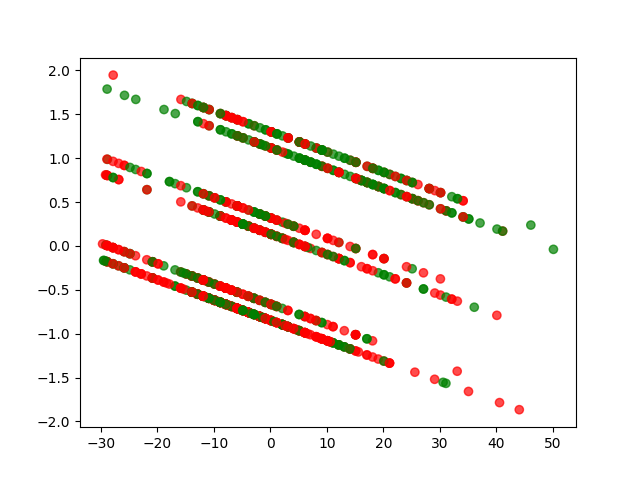
\includegraphics[scale=0.4]{titanic_acp}
\end{center}
\end{slide}

\begin{slide}{ACP}
\begin{center}
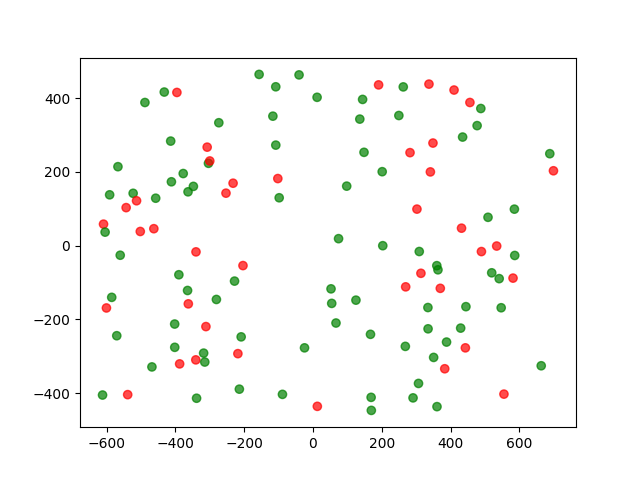
\includegraphics[scale=0.4]{titanic_acp_mv}
\end{center}
\end{slide}

\subsection{Approche non linéaire}

\begin{slide}{Kohonen Map}
\begin{center}
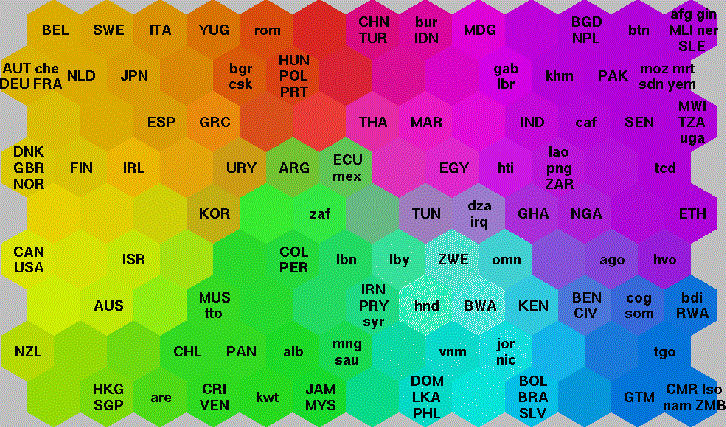
\includegraphics[scale=0.35]{povertymap}
\end{center}
\end{slide}

\begin{slide}{Kohonen Map}
\Pythonsmall{som1-extract}
\end{slide}

\begin{slide}{Kohonen Map}
\begin{center}
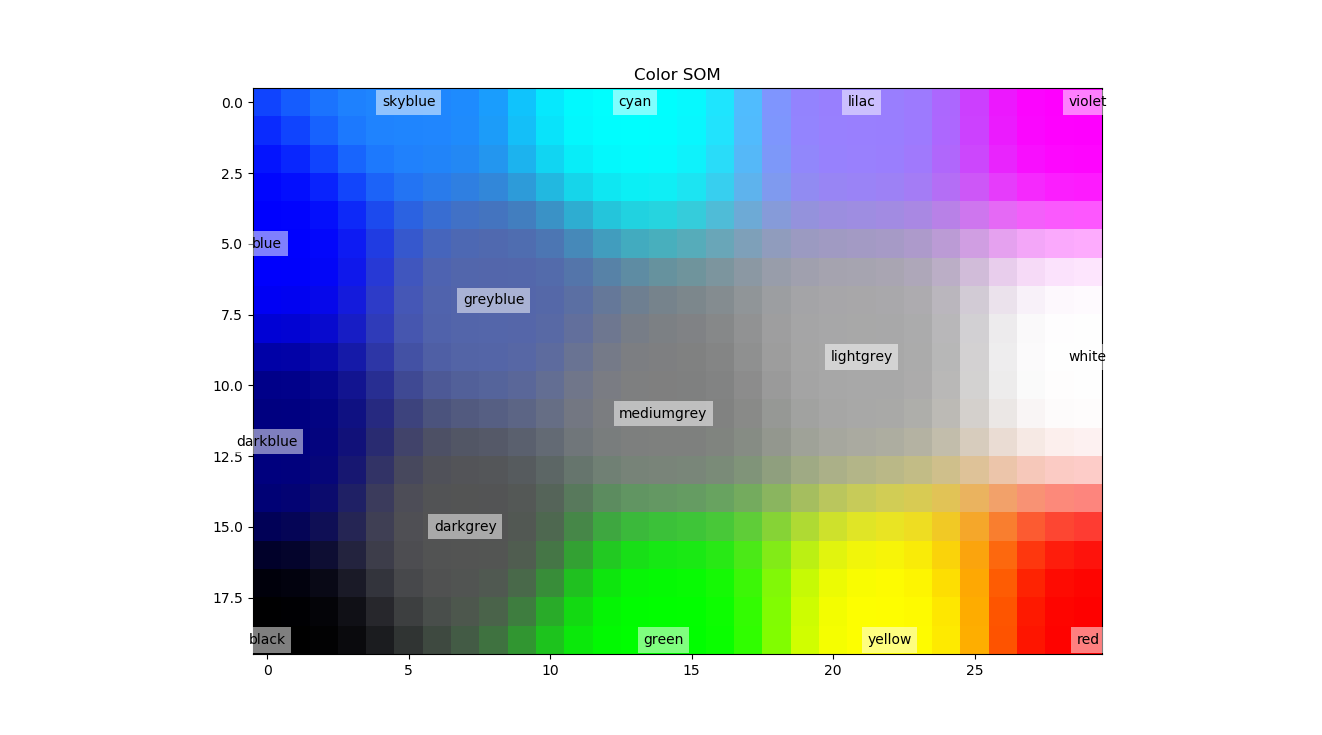
\includegraphics[scale=0.35]{som_exemple1}
\end{center}
\end{slide}

\section{Décision}

\subsection{Introduction}

\begin{slide}{Un graphe de compatibilité}

\begin{tikzpicture}

\node (1) at (0,0){Ainur};
\node (2) at (0,1){Béatrice};
\node (3) at (0,2){Claude};
\node (4) at (0,3){Denis};
\node (5) at (4,0){Eléonore};
\node (6) at (4,1){François};
\node (7) at (4,2){Genki};
\node (8) at (4,3){Hussein};
\draw (1) -- (5);
\draw (1) -- (7);
\draw (2) -- (5);
\draw (2) -- (6);
\draw (2) -- (8);
\draw (3) -- (6);
\draw (4) -- (6);
\draw (4) -- (8);

\end{tikzpicture}

\end{slide}

\begin{slide}{Une allocation sous-optimale}

\begin{tikzpicture}

\node (1) at (0,0){Ainur};
\node (2) at (0,1){Béatrice};
\node (3) at (0,2){Claude};
\node (4) at (0,3){Denis};
\node (5) at (4,0){Eléonore};
\node (6) at (4,1){François};
\node (7) at (4,2){Genki};
\node (8) at (4,3){Hussein};
\draw[ultra thick,red] (1) -- (5);
\draw (1) -- (7);
\draw (2) -- (5);
\draw[ultra thick,red] (2) -- (6);
\draw (2) -- (8);
\draw (3) -- (6);
\draw (4) -- (6);
\draw[ultra thick,red] (4) -- (8);

\end{tikzpicture}

\end{slide}

\begin{slide}{Une allocation optimale}

\begin{tikzpicture}

\node (1) at (0,0){Ainur};
\node (2) at (0,1){Béatrice};
\node (3) at (0,2){Claude};
\node (4) at (0,3){Denis};
\node (5) at (4,0){Eléonore};
\node (6) at (4,1){François};
\node (7) at (4,2){Genki};
\node (8) at (4,3){Hussein};
\draw (1) -- (5);
\draw[ultra thick,red] (1) -- (7);
\draw[ultra thick,red] (2) -- (5);
\draw (2) -- (6);
\draw (2) -- (8);
\draw[ultra thick,red] (3) -- (6);
\draw (4) -- (6);
\draw[ultra thick,red] (4) -- (8);

\end{tikzpicture}

\end{slide}

\begin{slide}{Pas toujours facile}
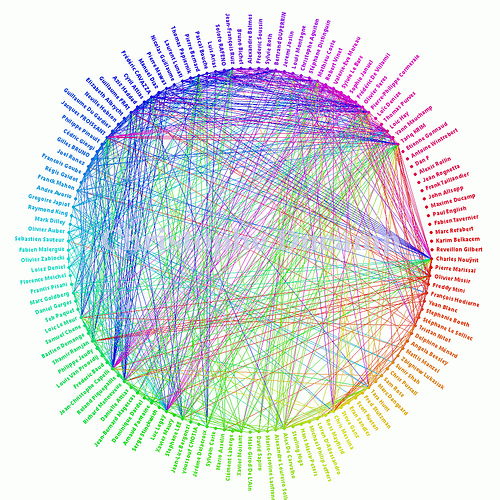
\includegraphics[scale=0.35]{facebookfriendwheel.jpg}
\end{slide}

\begin{slide}{Formalisation du problème}
Soit un graphe $G$ défini par un ensemble de sommets $V$ et un ensemble d'arêtes $E$. On cherche 

\vspace{0.5cm}

\pause

un sous-ensemble d'arêtes $F \subset E$:

\vspace{0.5cm}

\pause

tel que deux arêtes ne soient pas incidentes

\vspace{0.5cm}

\pause

de taille maximale

\end{slide}



\subsection{Ford-Fulkerson / Edmonds}

\begin{slide}{Chaîne augmentante}

\begin{tikzpicture}

\node (1) at (0,0){Ainur};
\node (2) at (0,1){Béatrice};
\node (3) at (0,2){Claude};
\node (4) at (0,3){Denis};
\node (5) at (4,0){Eléonore};
\node (6) at (4,1){François};
\node (7) at (4,2){Genki};
\node (8) at (4,3){Hussein};
\draw[ultra thick,red] (1) -- (5);
\draw (1) -- (7);
\draw (2) -- (5);
\draw[ultra thick,red] (2) -- (6);
\draw (2) -- (8);
\draw (3) -- (6);
\draw (4) -- (6);
\draw[ultra thick,red] (4) -- (8);

\end{tikzpicture}

\end{slide}

\begin{slide}{Deux sommets isolés}

\begin{tikzpicture}

\node (1) at (0,0){Ainur};
\node (2) at (0,1){Béatrice};
\node[shape=rectangle,fill=blue!40] (3) at (0,2){Claude};
\node (4) at (0,3){Denis};
\node (5) at (4,0){Eléonore};
\node (6) at (4,1){François};
\node[shape=rectangle,fill=blue!40] (7) at (4,2){Genki};
\node (8) at (4,3){Hussein};
\draw[ultra thick,red] (1) -- (5);
\draw (1) -- (7);
\draw (2) -- (5);
\draw[ultra thick,red] (2) -- (6);
\draw (2) -- (8);
\draw (3) -- (6);
\draw (4) -- (6);
\draw[ultra thick,red] (4) -- (8);

\end{tikzpicture}

\end{slide}

\begin{slide}{Une chaîne alternée}

\begin{tikzpicture}

\node (1) at (0,0){Ainur};
\node (2) at (0,1){Béatrice};
\node[shape=rectangle,fill=blue!40] (3) at (0,2){Claude};
\node (4) at (0,3){Denis};
\node (5) at (4,0){Eléonore};
\node (6) at (4,1){François};
\node[shape=rectangle,fill=blue!40] (7) at (4,2){Genki};
\node (8) at (4,3){Hussein};
\draw[ultra thick,red] (1) -- (5);
\draw[ultra thick,blue] (1) -- (7);
\draw[ultra thick,blue] (2) -- (5);
\draw[ultra thick,red] (2) -- (6);
\draw (2) -- (8);
\draw[ultra thick,blue] (3) -- (6);
\draw (4) -- (6);
\draw[ultra thick,red] (4) -- (8);

\end{tikzpicture}

\end{slide}

\begin{slide}{Chaîne augmentante}

\Python{testff}

\end{slide}

\begin{slide}{Le cas non-biparti}

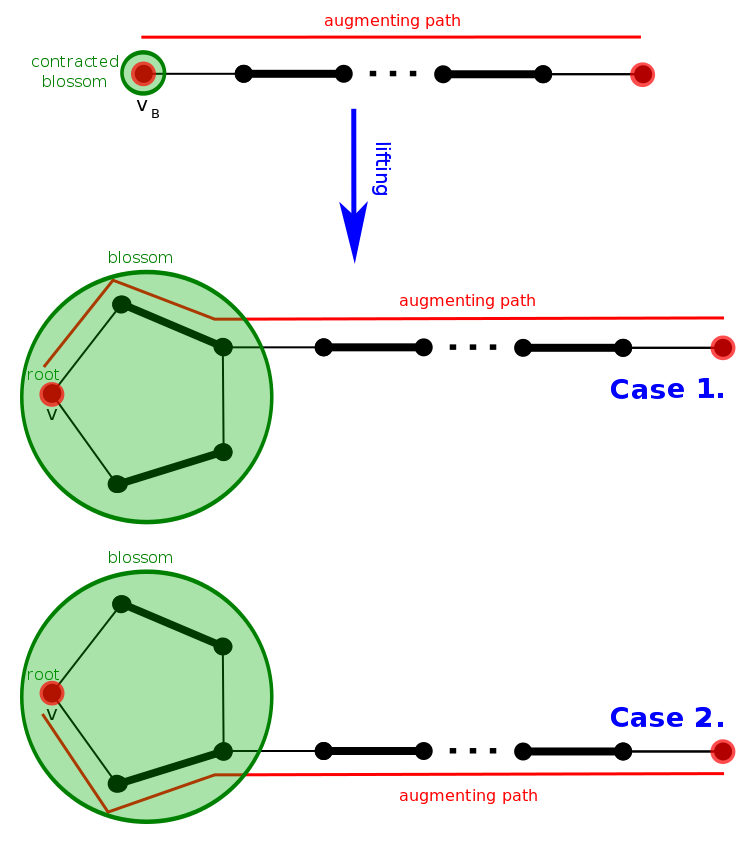
\includegraphics[scale=0.2]{Edmonds}

\end{slide}


\subsection{Construction du graphe}

\begin{slide}{Données monovariées}

\begin{tikzpicture}

\draw[-latex,thick] (-1,-1) -- (7,-1)node[below] {revenus};

\node[shape=rectangle,fill=red] (1) at (0,0){};
\node[shape=rectangle,fill=red] (2) at (1.8,0){};
\node[shape=rectangle,fill=red] (4) at (3,0){};
\node[shape=rectangle,fill=red] (4) at (3.4,0){};
\node[shape=rectangle,fill=red] (5) at (4.8,0){};
\node[shape=rectangle,fill=red] (6) at (6,0){};
\pause
\draw (1.6,0.3) rectangle (3.6,-0.3);
\draw (4.6,0.3) rectangle (6.2,-0.3);

\end{tikzpicture}

\end{slide}


\begin{slide}{Données bivariées}

\begin{tikzpicture}

\draw[-latex,thick] (-1,-1) -- (7,-1)node[below] {revenus};
\draw[-latex,thick] (-1,-1) -- (-1,4.5)node[left] {études};

\node[shape=rectangle,fill=red] (1) at (0,4){};
\node[shape=rectangle,fill=red] (2) at (1.8,1){};
\node[shape=rectangle,fill=red] (4) at (3,0.5){};
\node[shape=rectangle,fill=red] (4) at (3.4,3){};
\node[shape=rectangle,fill=red] (5) at (4.8,3.2){};
\node[shape=rectangle,fill=red] (6) at (6,1){};
\pause
\draw (1.6,1.3) rectangle (3.2,0.2);
\draw (3.2,2.7) rectangle (5,3.4);

\end{tikzpicture}

\end{slide}


\begin{slide}{Données multivariées}

Comment représenter sur un écran un classement selon des dizaines ou des milliers de critères ? 

\vspace{0.5cm}

Comment déterminer des compatibilités entre des individus représentés par autant de variables ?

\end{slide}

\begin{slide}{Réduction dimensionnelle}
\begin{center}
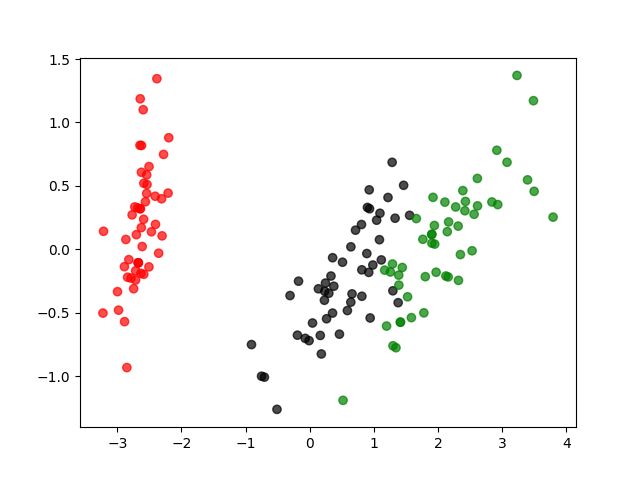
\includegraphics[scale=0.4]{iris_acp}
\end{center}
\end{slide}

\begin{slide}{Réduction dimensionnelle}
\begin{center}
\Python{acp}
\end{center}
\end{slide}


\begin{slide}{{\`A} vous de jouer !}

Importez le fichier \texttt{data2.csv} et essayez de construire une représentation ou de modéliser un graphe de compatibilité.

\end{slide}

\begin{slide}{Données numériques}

Normalisation (exemple) : 

$$x' = \frac{x-xmin}{xmax-xmin}$$

Agrégation (exemple) :

$$ d(X,Y) = \sqrt{\sum(x_i-y_i)^2} $$

\end{slide}

\begin{slide}{Données par modalités}

Distance binaire :

$$ d(X,Y) = \sharp \{ x_i \neq y_i \} = \sum_{x_i \neq y_i} 1 $$

Distance pondérée :

$$ d(X,Y) = \sum_{x_i \neq y_i} \omega_i $$

\end{slide}

\begin{slide}{Exemple}

$X$ : BLOND, BAC+5, MODEM, 43 ans

$Y$ : BLOND, BAC+2, NPA, 36 ans\\

\vspace{0.2cm}

\pause

$X'$ : BLOND, 0.6, MODEM, 0.7

$Y'$ : BLOND, 0.3, NPA, 0.55

\pause

$$d(X,Y) = \sqrt{0 + (0.6-0.3)^2 + 1 + (0.7-0.55)^2}$$

\end{slide}


\begin{slide}{{\`A} vous de jouer !}

Construisez une matrice de distances sur les données du fichier \texttt{data2.csv}.

\end{slide}

\begin{slide}{Principe}

On fixe un seuil, par exemple $S=N/4$, où $N$ est le nombre de variables.

\pause

On considère que deux sommets doivent être reliés si et seulement si leur distance est inférieure au seuil.

$(X,Y) \in G \Longleftrightarrow d(X,Y) < S$

\end{slide}

\begin{slide}{Exemple}

$X$ : BLOND, 0.6, MODEM, 0.7\\
$Y$ : BLOND, 0.3, NPA, 0.55\\
$Z$ : BRUN, 0.5, LR, 0.8\\
$T$ : BRUN, 0.2, NPA, 0.2\\

\end{slide}

\begin{slide}{Exemple}

\begin{tabular}{|c|c|c|c|c|}
\hline
& X & Y & Z & T \\ \hline
X &\cellcolor{black!20} \color{black!20} 0.0&1.45&2.30&2.90 \\ \hline
Y &&\cellcolor{black!20} \color{black!20} 0.0&2.45&1.45 \\ \hline
Z &&&\cellcolor{black!20} \color{black!20} 0.0&1.90 \\ \hline
T &&&&\cellcolor{black!20} \color{black!20} 0.0 \\ \hline
\end{tabular}

\end{slide}

\begin{slide}{Exemple}

\begin{tabular}{|c|c|c|c|c|}
\hline
& X & Y & Z & T \\ \hline
X &\cellcolor{black!20} \color{black!20} 0.0&\cellcolor{red!50}{1.45}&2.3&2.9 \\ \hline
Y &&\cellcolor{black!20} \color{black!20} 0.0&2.45&\cellcolor{red!50}1.45 \\ \hline
Z &&&\cellcolor{black!20} \color{black!20} 0.0&\cellcolor{red!50}1.9 \\ \hline
T &&&&\cellcolor{black!20} \color{black!20} 0.0 \\ \hline
\end{tabular}

\end{slide}


\begin{slide}{{\`A} vous de jouer !}

1) Fixez un seuil et utilisez la matrice de l'exercice précédent pour construire des proximités entre les individus. \\

\vspace{0.3cm}

2) Essayez de produire le graphe correspondant.

\end{slide}

\subsection{MATCHING vs CLUSTERING (cliques)}

\begin{slide}{Rappel : le MATCHING}
Soit un graphe $G$ défini par un ensemble de sommets $V$ et un ensemble d'arêtes $E$. On cherche 

\vspace{0.5cm}

\pause

un sous-ensemble d'arêtes $F \subset E$:

\vspace{0.5cm}

\pause

tel que deux arêtes ne soient pas incidentes

\vspace{0.5cm}

\pause

de taille maximale

\end{slide}


\begin{slide}{Rappel : le CLUSTERING}
Soit un graphe $G$ défini par un ensemble de sommets $V$ et un ensemble d'arêtes $E$. On cherche 

\vspace{0.5cm}

\pause

Une division de $V$ en sous-ensembles disjoints $V_1$, $V_2$, $V_3$...

\vspace{0.5cm}

\pause

avec un maximum d'arêtes à l'intérieur de chaque $V_i$

\vspace{0.5cm}

\pause

et un minimum à l'extérieur, entre les différents $V_i$.

\end{slide}

\begin{slide}{Exemple}

\begin{tikzpicture}

\node[shape=rectangle,fill=red] (1) at (0,0){};
\node[shape=rectangle,fill=red] (2) at (0,1){};
\node[shape=rectangle,fill=red] (3) at (1,2){};
\node[shape=rectangle,fill=red] (4) at (2,1){};
\node[shape=rectangle,fill=red] (5) at (4,2){};
\node[shape=rectangle,fill=red] (6) at (5,3){};
\node[shape=rectangle,fill=red] (7) at (6,2.5){};
\node[shape=rectangle,fill=red] (8) at (7,1){};
\node[shape=rectangle,fill=red] (9) at (5.5,1.5){};
\draw (1) -- (2);
\draw (1) -- (3);
\draw (2) -- (3);
\draw (3) -- (4);
\draw (3) -- (5);
\draw (4) -- (1);
\draw (5) -- (6);
\draw (5) -- (7);
\draw (7) -- (8);
\draw (6) -- (9);
\draw (5) -- (9);
\pause
\draw[dashed] (-0.3,-0.3) rectangle (2.3,2.3);
\draw[dashed,color=red] (3.7,3.3) rectangle (5.8,1.2);
\draw[dashed] (5.7,2.8) rectangle (7.3,0.7); 

\end{tikzpicture}

\end{slide}

\begin{slide}{Différents types d'objectifs}

\begin{itemize}
\item Ne regrouper que des éléments tous deux à deux compatibles : 

$$x \in V_i, y \in V_i \Longrightarrow (x,y) \in G $$

\pause

\item Ratio inter/intra minimal :

$$ \min \frac{\sharp\{(x,y) \in G, x \in V_i, y \in V_j\}}{\sharp\{(x,y) \in G, x,y \in V_i\}}$$

\end{itemize}

\end{slide}


\begin{slide}{{\`A} vous de jouer !}

Trouvez un clustering pertinent sur l'exemple des exercices précédents.

\end{slide}


\subsection{La classification hiérarchique ascendante}

\begin{slide}{Principe}

On va procéder de façon itérative.

\pause

A chaque étape on regroupe les deux éléments les plus proches.

\pause

Le groupement ainsi constitué est considéré comme un pseudo-élément positionné en son barycentre.

\end{slide}


\begin{slide}{Exemple}

\begin{tikzpicture}

\node[shape=rectangle,fill=red] (1) at (0,0){};
\node[shape=rectangle,fill=red] (2) at (0,1){};
\node[shape=rectangle,fill=red] (3) at (1,2){};
\node[shape=rectangle,fill=red] (4) at (2,1){};
\node[shape=rectangle,fill=red] (5) at (4,2){};
\node[shape=rectangle,fill=red] (6) at (5,3){};
\node[shape=rectangle,fill=red] (7) at (6,2.5){};
\node[shape=rectangle,fill=red] (8) at (7,1){};
\node[shape=rectangle,fill=red] (9) at (5.5,1.5){};
\pause
\draw[dashed] (-0.3,-0.3) rectangle (0.3,1.3);
\pause
\draw[dashed] (4.7,2.2) rectangle (6.3,3.3);

\end{tikzpicture}

\end{slide}

\begin{slide}{Exemple}

\begin{tikzpicture}

\node[shape=rectangle,fill=red] (1) at (0,0){};
\node[shape=rectangle,fill=red] (2) at (0,1){};
\node[shape=rectangle,fill=red] (3) at (1,2){};
\node[shape=rectangle,fill=red] (4) at (2,1){};
\node[shape=rectangle,fill=red] (5) at (4,2){};
\node[shape=rectangle,fill=red] (6) at (5,3){};
\node[shape=rectangle,fill=red] (7) at (6,2.5){};
\node[shape=rectangle,fill=red] (8) at (7,1){};
\node[shape=rectangle,fill=red] (9) at (5.5,1.5){};
\draw[dashed] (-0.3,-0.3) rectangle (0.3,1.3);
\draw[dashed] (4.7,1.2) rectangle (6.3,3.3);
\pause
\draw[dashed] (0.7,0.7) rectangle (2.3,2.3);

\end{tikzpicture}

\end{slide}

\begin{slide}{Exemple}

\begin{tikzpicture}

\node[shape=rectangle,fill=red] (1) at (0,0){};
\node[shape=rectangle,fill=red] (2) at (0,1){};
\node[shape=rectangle,fill=red] (3) at (1,2){};
\node[shape=rectangle,fill=red] (4) at (2,1){};
\node[shape=rectangle,fill=red] (5) at (4,2){};
\node[shape=rectangle,fill=red] (6) at (5,3){};
\node[shape=rectangle,fill=red] (7) at (6,2.5){};
\node[shape=rectangle,fill=red] (8) at (7,1){};
\node[shape=rectangle,fill=red] (9) at (5.5,1.5){};
\draw[dashed] (-0.3,-0.3) rectangle (0.3,1.3);
\draw[dashed] (3.7,1.2) rectangle (6.3,3.3);
\draw[dashed] (0.7,0.7) rectangle (2.3,2.3);

\end{tikzpicture}

\end{slide}

\begin{slide}{{\`A} vous de jouer !}

Programmez un algorithme de classification hiérarchique ascendante. Testez-le sur l'exemple précédent (à partir de la table de distances).

\end{slide}

\section{Qualité d'un modèle}

\subsection{Différentes sources d'erreur}

\begin{slide}{Dissimilarité}

Choix d'une mesure de l'écart entre prédiction et observation.\\
\pause
Minimiser :
$$d(\tilde{f}(x),y)$$

\end{slide}

\begin{slide}{Exemples de dissimilarités}

$$d(\tilde{f}(x),y) = ||\tilde{f}(x)-y||_2^2 = \sum (\tilde{f}(x)_i-y_i)^2 $$

$$d(\tilde{f}(x),y) = |\tilde{f}(x)-y| = \sum |\tilde{f}(x)_i-y_i| $$

$$d(\tilde{f}(x),y) = |\{i,\tilde{f}(x)_i \neq y\}_i| $$

$$d(\tilde{f}(x),y) = \sum w_i|\tilde{f}(x)_i-y_i| $$

$$d(\tilde{f}(x),y) = \sum \phi_i(\tilde{f}(x)_i,y_i) $$

\end{slide}

\begin{slide}{Exercice}

\begin{exercice}
Trouvez des contextes pour lesquels des mesures de dissimilarités différentes sont appropriées.
\end{exercice}

\end{slide}


\begin{slide}{Rappel des Hypothèses}
Observations :\\

\begin{itemize}

\item Variable empirique cible $\tilde{Y}$
\item Variables empiriques explicatives $\tilde{X}$

\end{itemize}

\pause

Hypothèses :\\

\begin{itemize}

\item $\tilde{X}$ est un ensemble d'observations lié à un processus aléatoire $X$
\item $\tilde{Y}$ est un ensemble d'observations lié à un processus aléatoire $Y$
\item il existe une relation $Y = f(X)$

\end{itemize}

\pause

Objectifs :\\

\begin{itemize}
\item Produire une fonction $\tilde{f}$ à partir de $\tilde{X}$ et $\tilde{Y}$
\item Telle que $\tilde{f}$ soit une approximation fiable de $f$
\item On pourra ainsi prédire $\tilde{Y}' = \tilde{f}(\tilde{X}')$ sur un nouvel échantillon 
\end{itemize}

\end{slide}


\begin{slide}{Erreur du modèle}

La bonne mesure serait de minimiser :

$$D(\tilde{f}) = \mathbb{E}(d(\tilde{f}(x),y))$$

\pause

Mais comme on ne connaît pas la loi de $(X,Y)$ c'est impossible.

\end{slide}


\begin{slide}{Erreur moyenne empirique}

On dispose d'un échantillon de test $\tau = (X_j,Y_j)_{j\leq n}$.\\

Minimiser :
$$\tilde{D}(\tilde{f},\tau) = \frac{1}{n}\sum_{j \leq m} d(\tilde{f}(x_j),y_j)$$

\pause

Ne pas confondre cette somme sur les données avec la somme sur les variables !\\
Ne pas confondre cette moyenne empirique avec la moyenne 
\end{slide}

\begin{slide}{Convergence}

D'après la loi des grands nombres, si les observations de test sont indépendantes, la moyenne empirique converge vers l'erreur du modèle.
\end{slide}

\begin{slide}{Pertinence du test}
On cherche à évaluer la probabilité que l'écart entre les deux mesures soit faible.

$$P\left(\tilde{D}(\tilde{f},\tau)-D(\tilde{f}) > \epsilon \right) < 1 - \rho$$

\end{slide}

\subsection{Complexité}

\begin{slide}{Exponentielle rapide}
\begin{exercice}
Implémentez une fonction exponentielle. Combien de multiplications effectue-t-elle pour calculer $3^{130}$ ?
\end{exercice}
\end{slide}

\begin{slide}{Exponentielle rapide}
\Python{fastexp}
\end{slide}


\begin{slide}{Exemples d'algorithmes}

Exponentielle rapide : $O(\log n)$\\
Tri rapide, exponentielle naïve : $O(n)$\\
Tri par insertion : $O(n^2)$\\
Multiplication matricielle naïve : $O(n^3)$\\
{\'E}numération des sous-ensembles : $O(2^n)$\\
Voyageur de commerce, Coloration : $O(2^n)$\\
{\'E}numération des permutations : $O(n!)$

\end{slide}

\begin{slide}{Ordres de grandeur}
\begin{center}
\begin{tabular}{c|c|c|c}
Taille  & $n\log n$ & $n^3$ & $2^n$ \\
\hline
$n=20$ & $60$ & $8 000$ & $1 048 576$ \\
$n=50$ & $196$ & $125 000$ & $1 125 899 907 000 000$ \\
$n=100$ & $461$ & $1 000 000$ & $1 267 650 600 000 000 000 000 000 000 000$\\
\end{tabular}
\end{center}

\end{slide}

\begin{slide}{retour aux classifications}
\begin{exercice}
Quelle est la complexité d'un clustering en force brute ? Et celle d'une classification hiérarchique ascendante ?
\end{exercice}
\end{slide}



\end{document}